\documentclass{article}

% Language setting
\usepackage[english]{babel}

% Set page size and margins
\usepackage[letterpaper,top=2cm,bottom=2cm,left=3cm,right=3cm,marginparwidth=1.75cm]{geometry}

\usepackage{amsmath}
\usepackage{graphicx}
\usepackage[colorlinks=true, allcolors=blue]{hyperref}

\title{Reference Manual for TwoDSensorModule}
\author{Hojae Lee}

\begin{document}
\maketitle
\tableofcontents

\section{Introduction}

This document is a reference manual for
\href{https://github.com/thousandbrainsproject/tbp.monty}{\texttt{TwoDSensorModule}}
as implemented in \texttt{tbp.monty} version \texttt{0.33.0}. It is written
for future maintainers and contributors who need to improve the 2D sensor
module without losing the design intent behind the current implementation. The
goal is to explain what problem each algorithm solves, why the main choices
were made, what limitations remain, and where future work can build on the
existing design.

\texttt{TwoDSensorModule} converts local surface observations into a
2D-compatible representation while preserving compatibility with Monty's
message interface. It has two central responsibilities. First, it detects the
dominant texture-edge orientation in an image patch so a local visual edge can
be represented as pose information. Second, it accumulates movement over a
curved surface in a transported 2D surface chart while still emitting
3D-shaped location and displacement fields.

The implementation of \texttt{TwoDSensorModule} is divided into two main
parts:

\begin{enumerate}
  \item Estimating dominant texture-edge orientation in a sensor patch.
  \item Accumulating 2D movement over a curved surface.
\end{enumerate}

% The manual is also expected to grow with a results-oriented section. That
% section should add qualitative edge-detection examples, parameter studies,
% learned and projected edge models, 2D movement behavior, and inference
% comparisons. The commented outline below preserves the current working list of
% result topics and related Shortcut tickets.

% The edge-detection section explains the image-gradient and structure-tensor path
% used to estimate edge orientation in image space. The 2D movement section
% explains tangent-frame transport and arc-length correction for movement on
% curved surfaces. The final integration
% section explains how \texttt{TwoDSensorModule.step} combines the saved surface
% geometry, optional texture-edge pose, and 2D location/displacement convention
% into one outgoing Monty message.

% Comment: Do not delete the outline below. We will need to add results (I think before methods? not sure yet), the below lists some relevant Shortcut tickets that contain these. 
% Outline for Results:
% 1. Include example patches of detected edges - draw main object, and then "zooming" into specific patches. 
% 2. Include example of different zooms and blur factors (https://app.shortcut.com/thousandbrainsproject/story/2743/weighted-algorithm-on-monty)
% 3. Include example of projected / learned models (edge as vector) - TBP Disk and Numenta Disk (https://app.shortcut.com/thousandbrainsproject/story/2190/ensure-edge-is-represented-as-morphological-feature-and-can-be-placed-within-3d-space)
% 4. Include results on synthetic images to demonstrate various parameters of EdgeDetection class 
% - https://app.shortcut.com/thousandbrainsproject/story/2666/evaluate-additional-synthetic-objects-conditions
% 5. Edge within edge (https://app.shortcut.com/thousandbrainsproject/story/2667/edge-within-edge-see-viviane-s-share-on-slack-can-we-learn-a-hierarchical-model-with-a-low-level)
% 6. 2D movement
% 6. Inference results 
% 7. https://app.shortcut.com/thousandbrainsproject/story/3707/qualitatively-estimate-spacing-error-and-inference-accuracy-when-generalizing-between-2d-models-learned-on-different-surface
% https://app.shortcut.com/thousandbrainsproject/story/3700/compare-2d-on-2d-vs-3d-on-3d-inference-when-agent-translated-but-using-burst-sampling
% 8. Setting surface normal to Z: https://app.shortcut.com/thousandbrainsproject/story/4583/update-2d-sm-with-pose-fully-defined-false-if-no-edge-and-rotating-standard-bases-instead-of-using-surface-normal

\section{Detecting Dominant Texture-Edge Orientation in a Patch}
\label{edge_detection}

The goal of the edge-detection work was to detect the dominant texture-edge orientation in an image patch.
Once detected, the edge orientation is projected into the 2D tangent frame used by \texttt{TwoDSensorModule} (see Section~\ref{sec:tangent_frame}).
Unlike some other features in Monty, which are read directly from the center pixel of a $64 \times 64$ patch, we wanted to extract the dominant orientation across the \textit{whole} patch.
This led to the development of \texttt{EdgeDetector} (in \texttt{edge\_detection.py}), which extracts an edge angle between $(0, \pi]$ when a dominant edge is identified, along with supporting edge attributes.
The Edge Detection module also provides a helper for projecting the detected image-space edge angle into the vectors expected by the chosen reference frame.

% TODO: Add a figure demonstrating examples and desired properties of this
% problem: centered edge, off-center edge, multiple competing edges, and the
% same texture at different zoom levels.
% TODO: Add a figure illustrating the desired specification of edge detection.
% Figure caption draft: A texture edge can pass near the center, occupy only
% part of the patch, appear together with weaker secondary edges, or change
% apparent dominance as zoom changes.

\subsection{Patch-Level Edge Detection Pipeline}

In computer vision, one common way to detect an edge at the pixel level is to analyze changes in image gradients along the $x$- and $y$-directions.
The Canny edge detector is an example of this kind of gradient-based method~\cite{opencv_canny}.

To aggregate gradient information across a whole patch, we use the structure tensor, a compact summary of local gradient variation~\cite{khan_corner_detection,opencv_gst}.
The structure tensor lets us aggregate gradient evidence across pixels in a controlled way instead of relying on a single center-pixel gradient.

% TODO: A small figure showing how edge angle is measured (image-x to image-y).

The following describes the main algorithm implemented in \texttt{EdgeDetector}.
Given a \texttt{SensorObservation}, the detector first extracts the $(64, 64, 3)$ RGB patch and converts it to grayscale.
The current Monty implementation stores \texttt{observation["rgba"]} in red-green-blue order, but users should be careful if they are using an alternate approach such as constructing images via OpenCV, as OpenCV's \texttt{cv2.imread} returns blue-green-red (BGR) images.
Passing BGR data into \texttt{cv2.COLOR\_RGB2GRAY} changes the grayscale values that drive the gradient calculation.

From the grayscale image, the \texttt{EdgeDetector} computes Sobel gradients $I_x$ (gradient in the $x$-direction) and $I_y$ (gradient in the $y$-direction).
From these gradients, we can build a structure tensor for each pixel of our $64 \times 64$ patch as follows:
\[
  J =
  \begin{bmatrix}
    I_x^2 & I_x I_y \\
    I_x I_y & I_y^2
  \end{bmatrix}
\]

The per-pixel structure tensors are then reduced to a single aggregated $2 \times 2$ matrix for the entire patch using a center-biased weighted average, as Monty generally extracts features near the center of a sensor patch.
The weight for each pixel is calculated as the product of Gaussian radial weighting (which gives more importance to center pixels) and gradient energy (which gives more importance to clear, strong edges).

From the aggregated structure tensor, the dominant gradient angle can be computed using:
\[
  \theta_\text{gradient} =
    \frac{1}{2}
    \operatorname{atan2}(2 * J_{xy}, J_{xx} - J_{yy})
\]
The edge angle is perpendicular to this gradient direction:
\[
  \theta_\text{edge} = \theta_\text{gradient} + \frac{\pi}{2}
\]
This results in detected edge angle in the range of $\theta_\text{edge} \in (0, \pi]$. Note that for horizontal lines, the edge angle is always resolved to $\pi$ rather than $0$ because NumPy's \texttt{arctan2(+0.0, negative)} returns $\pi$ under IEEE 754 signed-zero behavior (the first argument is \texttt{+0.0} because an ideal horizontal line has no horizontal-gradient component, so the cross term $J_{xy}=I_x I_y$ aggregates to zero; the second argument is negative because vertical gradient energy dominates, making $J_{xx} - J_{yy} < 0$)~\cite{numpy_arctan2}.

Besides the edge angle, we extract two useful edge attributes from the aggregated structure tensor that represents the quality of detected edges: coherence and edge strength. As a $2 \times 2$ positive semi-definite matrix~\cite{wikipedia_definite_matrix}, the aggregated structure tensor has two eigenvalues $\lambda_{\max}$, $\lambda_{\min} \geq 0$.
A clean straight edge has one large eigenvalue and one small eigenvalue; a corner, junction, or isotropic texture has two similar eigenvalues because gradient energy exists in multiple directions. This is captured in the attribute \texttt{"coherence"}, which is defined as:

\[
  \text{coherence} = \frac{\lambda_{\max} - \lambda_{\min}}
       {\lambda_{\max} + \lambda_{\min}}
\]
Note that coherence has a range of $[0, 1]$ and values closer to 1 indicate presence of a clear edge. In Monty, only edges whose $\text{coherence} > 0.5$ is considered to be a true detected edge by default, though this can be adjusted by setting the \texttt{coherence\_threshold} for \texttt{EdgeDetector} in configurations.

Next, edge strength is defined as $\sqrt{\lambda_{\max}}$, and indicates the dominant gradient magnitude scale of the patch~\cite{khan_corner_detection,opencv_gst}. The example patches below should span different coherence and edge-strength values to give a qualitative sense of how these scores change across weak texture, clean straight edges, corners, and ambiguous gradient evidence.

\begin{figure}[h]
  \centering
  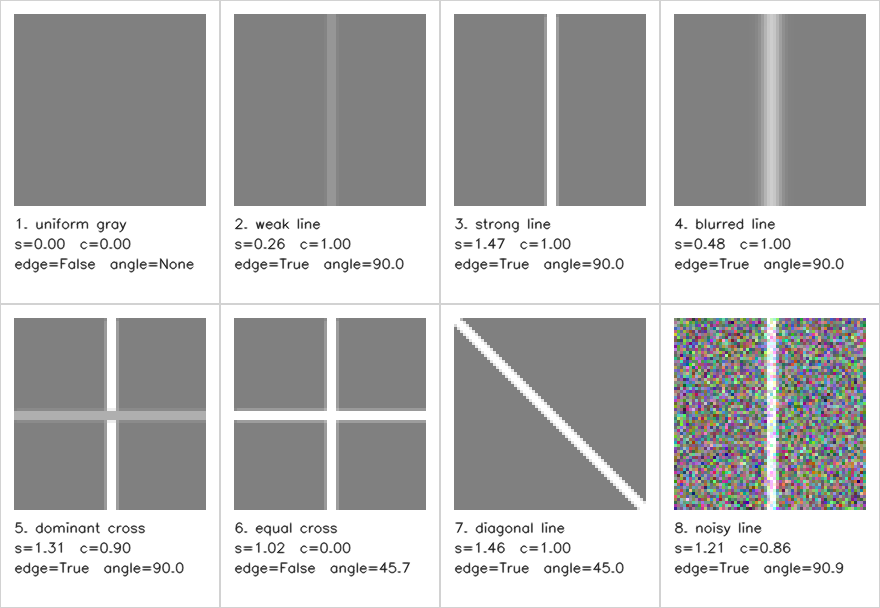
\includegraphics[width=\textwidth]{../figures/edge_quality_examples/edge_quality_contact_sheet.png}
  \caption{Synthetic 64x64 texture patches illustrating how \texttt{EdgeDetector}
  reports edge strength and coherence for weak, clean, blurred, ambiguous, and
  noisy line evidence. Scores are measured by the current implementation using
  the default detector parameters.}
  \label{fig:edge-quality-examples}
\end{figure}

Finally, \texttt{EdgeDetector} checks whether the detected RGB edge corresponds to a depth discontinuity, as we want to extract texture edges on a surface (e.g. logo on a mug), rather than object boundaries (e.g. mug against black void).
To perform this check, it computes gradients on the depth patch and projects that gradient onto the direction perpendicular to the detected edge.
If the depth gradient is above the default \texttt{depth\_edge\_threshold} of \texttt{0.01} meters, it indicates depth is changing rapidly across the detected edge and sets \texttt{is\_geometric\_edge} to \texttt{true}; this depth cutoff and the main RGB edge-detection parameters are summarized in Table~\ref{tab:edge-detector-parameters}.

% TODO: Add diagram / sketch of how geometric edge results in "no edge".

\begin{table}[ht]
  \centering
  \begin{tabular}{p{0.25\linewidth} p{0.13\linewidth} p{0.50\linewidth}}
    \hline
    Parameter & Default & Description \\
    \hline
    \texttt{kernel\_size} & \texttt{7} & Gaussian smoothing of the per-pixel tensor field. \\
    \texttt{radius} & \texttt{14.0} & Radius of the center-biased weighting window suitable for $64 \times 64$ patch. \\
    \texttt{sigma\_r} & \texttt{7.0} & Falloff of the radial Gaussian weight; downweights peripheral gradients smoothly, with an empirical default. \\
    \texttt{coherence\_threshold} & \texttt{0.5} & Minimum orientation coherence for a detected edge; a middle-of-range requirement on a score bounded in $[0, 1]$. \\
    \texttt{strength\_threshold} & \texttt{0.1} & Minimum gradient strength for a detected edge; intentionally low so weak but coherent texture edges can still pass. \\
    \texttt{depth\_edge\_threshold} & \texttt{0.01} & Minimum perpendicular depth change for marking a detected RGB edge as geometric, assuming depth is measured in meters. \\
    \hline
  \end{tabular}
  \caption{Default \texttt{EdgeDetector} parameters.}
  \label{tab:edge-detector-parameters}
\end{table}

\begin{table}[ht]
  \centering
  \begin{tabular}{p{0.24\linewidth} p{0.18\linewidth} p{0.46\linewidth}}
    \hline
    Field & Type & Meaning \\
    \hline
    \texttt{angle} & float or \texttt{None} & Estimated dominant edge orientation; \texttt{None} when no reliable orientation was computed. \\
    \texttt{strength} & float & Dominant gradient magnitude scale, computed from $\sqrt{\lambda_{\max}}$. \\
    \texttt{coherence} & float & Orientation quality score in $[0, 1]$. \\
    \texttt{is\_geometric\_edge} & bool & Whether the RGB edge also appears to be a depth discontinuity. \\
    \texttt{has\_edge} & bool & Final detector decision after strength and coherence thresholds. \\
    \hline
  \end{tabular}
  \caption{\texttt{EdgeFeatures} fields returned by \texttt{EdgeDetector}.}
  \label{tab:edge-features}
\end{table}

A limitation of \texttt{EdgeDetector} is that it returns one dominant orientation per patch.
If the patch contains more than one edge, the aggregated structure tensor may return a compromise orientation rather than one of the visible edges.
This can happen when two edges have similar strength, when a corner or junction fills the center of the patch, or when an off-center strong edge competes with the center-biased target edge.
In the current experiments, a zoom value of \texttt{30} is used to reduce this ambiguity by making the camera patch cover a smaller surface neighborhood, increasing the chance that each patch contains only one dominant texture edge.
This is an empirical mitigation rather than a formal guarantee: repeated or high-frequency texture can still put multiple useful edges in one patch.

\subsection{Projecting Image-Space Edge Orientation into 2D Pose}

The \texttt{angle} field in Table~\ref{tab:edge-features} is still an image-space measurement: it is measured from the image x-axis toward the image y-axis, i.e., downward in the image.
To use that angle as a pose feature, \texttt{TwoDSensorModule} must express the detected edge in the module's transported local 2D coordinates.
\texttt{\_angle\_to\_pose\_2d} performs this adapter step by converting the image-space edge angle into pose vectors in the current \texttt{TangentFrame}; readers unfamiliar with that moving local basis may want to read Section~\ref{sec:tangent_frame} first.

The conversion starts by mapping the image axes into world coordinates:
\[
  x_{\mathrm{img}}^{w} = R[1, 0, 0]^T,
  \quad
  y_{\mathrm{img}}^{w} = R[0, -1, 0]^T
\]
where $R$ is the rotation component of \texttt{cam\_to\_world}.
The negative sign in the image-y basis is load-bearing: image coordinates have positive y downward, while the camera/world convention used here treats positive y in the opposite (or upward) direction.

The edge angle then becomes a world-space direction:
\[
  e^w =
    \cos(\theta) x_{\mathrm{img}}^{w}
    + \sin(\theta) y_{\mathrm{img}}^{w}
\]
This vector still lives in 3D camera/world geometry, so the function projects it onto the local surface tangent plane, normalizes it, and expresses it in the transported tangent basis:
\[
  e^{2d} =
  \begin{bmatrix}
    e^w \cdot u \\
    e^w \cdot v \\
    0
  \end{bmatrix}
\]
where $u$ and $v$ are \texttt{tangent\_frame.basis\_u} and \texttt{tangent\_frame.basis\_v}.
The returned pose vectors use that local edge tangent as the second row:
\[
  \begin{bmatrix}
    0 & 0 & 1 \\
    e_x^{2d} & e_y^{2d} & 0 \\
    -e_y^{2d} & e_x^{2d} & 0
  \end{bmatrix}
\]
The first row is the 2D model's normal.
The second row is the edge tangent in local 2D coordinates.
The third row is the in-plane perpendicular that completes a right-handed local pose.

Callers that need a world-space tangent vector should use a separate helper rather than treating this returned pose as a world-coordinate orientation.
More generally, any future reusable helper for \texttt{CameraSM} or another sensor module should make the target reference frame explicit: the edge orientation must be projected into the same frame in which the downstream learning module will later compare it.
The reusable pattern is:

\begin{verbatim}
def image_angle_to_frame_vector(
    angle,
    cam_to_world,
    frame_axis_1,
    frame_axis_2,
    frame_axis_3,
):
    R = cam_to_world[:3, :3]
    image_x_world = R @ np.array([1.0, 0.0, 0.0])
    image_y_world = R @ np.array([0.0, -1.0, 0.0])

    edge_world = (
        np.cos(angle) * image_x_world
        + np.sin(angle) * image_y_world
    )
    edge_world = project_onto_tangent_plane(edge_world, frame_axis_3)

    if np.linalg.norm(edge_world) < DEFAULT_TOLERANCE:
        return None

    edge_world = normalize(edge_world)

    # Return 2D coordinates in the requested frame. Callers that need Monty's
    # pose_vectors contract can use this vector to construct a 3x3 pose matrix.
    return np.array([
        np.dot(edge_world, frame_axis_1),
        np.dot(edge_world, frame_axis_2),
    ])
\end{verbatim}
Here, \texttt{frame\_axis\_1} and \texttt{frame\_axis\_2} are the two target-frame axes used for the returned coordinates.
\texttt{frame\_axis\_3} is the frame normal, which defines the plane in which the edge direction should be compared.
The helper deliberately returns only the 2D edge vector.
For \texttt{TwoDSensorModule}, that vector is then embedded into Monty's expected \(3 \times 3\) \texttt{pose\_vectors} shape as a normal, edge tangent, and in-plane perpendicular.

\section{Implementing 2D Movement}

The edge pipeline defines an orientation feature at a single contact point.
The movement pipeline defines how successive contacts become a 2D path on the object's surface.
Two pieces make that possible: \texttt{TangentFrame} keeps a moving local coordinate system attached to the surface, and the arc-length correction helpers convert projected 3D steps into distances along the curved surface.

\subsection{Maintaining a Moving Local Frame}
\label{sec:tangent_frame}

As the 2D sensor moves across a curved 3D surface, its tangent plane changes from point to point.
A fixed world-frame pair of axes can describe motion on a flat plane, but it cannot stay attached to a curved surface.
\texttt{TangentFrame} stores the moving local chart used by the 2D sensor: a right-handed orthonormal basis $(u, v, n)$, where $n$ is the current surface normal and $u$ and $v$ span the local tangent plane.

The initial normal determines the tangent plane, but it does not determine a unique pair of in-plane axes.
The constructor therefore chooses an arbitrary reference axis $a = [0, 1, 0]$ and falls back to $a = [0, 0, 1]$ when the reference axis is nearly parallel to the normal.
It then builds the basis with cross products:
\begin{align*}
  u &= \mathrm{normalize}(a \times n) \\
  v &= \mathrm{normalize}(n \times u)
\end{align*}
These cross products put $u$ and $v$ in the tangent plane and make $(u, v, n)$ right-handed.
The fallback axis only prevents a degenerate cross product; it does not make the initial 2D coordinate system canonical.
Two episodes that start on different surface points can therefore begin with tangent frames that are rotated relative to one another.

\begin{figure}[h]
  \centering
  \includegraphics[width=0.8\textwidth]{../figures/tangent_frame_init.png}
  \caption{Initialization of the orthonormal tangent frame $(u, v, n)$ from a surface normal $n$.}
\end{figure}

When the sensor reaches a new surface point, \texttt{transport(new\_normal)} moves the existing basis to the new tangent plane by the minimum rotation that maps the old normal $n$ to the new normal $n'$.
If the normals are not parallel, the code constructs that rotation from the axis-angle representation:
\[
  \text{axis} = \mathrm{normalize}(n \times n'),
  \quad
  \theta = \arccos(n \cdot n')
\]
and applies the resulting rotation to $u$.
This keeps $u$ as close as possible to its previous direction while moving it into the new tangent plane, which is the discrete analogue of parallel transport.

After the rotation, the frame is re-orthonormalized.
This final projection is load-bearing: repeated small transports accumulate floating-point error, and re-orthonormalization keeps the frame aligned with the current normal over long trajectories.
If the new normal is parallel to the old normal, the rotation step is skipped, but re-orthonormalization still runs so that the stored frame remains aligned with the supplied normal.

\begin{figure}[h]
  \centering
  \includegraphics[width=0.6\textwidth]{../figures/tangent_frame_transport.png}
  \caption{Parallel transport of the tangent frame from normal $n$ to a new normal $n'$.}
\end{figure}

\subsection{Correcting Surface Displacement for Curvature}

The tangent frame gives each step a local 2D direction, but the raw displacement in that frame is still a tangent-plane projection.
On a curved surface, that projection is a chord-like measurement: it is shorter than the distance traveled along the surface itself.
Without a correction, the accumulated 2D path is systematically compressed on curved regions because each step records the flat projection rather than the surface arc.

\texttt{arc\_from\_projection} treats the surface locally as an osculating circle in the direction of motion.
The circle has the same tangent and normal curvature $k$ as the surface at the current point, so it gives a local approximation of how a tangent-plane projection $p$ relates to a surface arc length $s$.
Under that constant-curvature approximation:
\[
  p = \frac{\sin(k \cdot s)}{k}
  \quad\Longrightarrow\quad
  s = \frac{\arcsin(k \cdot p)}{k}
\]
The correction preserves the sign of the original projected displacement, so forward and backward movement along the same local direction remain distinguishable.
Using the magnitudes of curvature and projected displacement also means convex and concave curvature use the same arc-to-projection geometry.

Two regimes bypass the correction.
If $|k \cdot p| < 0.001$, the local surface is effectively flat over the step, so $\arcsin(kp) \approx kp$ and the function returns the original projection.
If $|k \cdot p| \geq 1.0$, the projection is outside the valid arcsine domain for this circle model.
Geometrically, the projected step is at least as large as the radius of curvature, so the constant-curvature local model is no longer a reliable description of the step.
In that case the function logs a warning and returns the original projection; the higher-level remedy is to take smaller 3D steps.

The remaining question is which curvature $k$ to use for a displacement direction that is not exactly aligned with a principal curvature direction.
\texttt{directional\_curvature} answers that with Euler's curvature formula.
Given principal curvatures $k_1, k_2$ and their corresponding directions $\hat{d}_1, \hat{d}_2$:
\[
  k(\theta) = k_1 \cos^2\theta + k_2 \sin^2\theta
\]
where $\theta$ is the angle between the movement direction and $\hat{d}_1$.
The helper validates that the principal curvature directions are unit, orthogonal vectors and that the movement direction lies in their plane before applying the formula.
A zero movement direction returns zero curvature because no directional correction is needed.

\texttt{arc\_length\_corrected\_displacement} ties the two pieces together for a step represented in the transported tangent frame.
Given projected displacements $(du, dv)$ along basis vectors $(u, v)$, it computes the normal curvature in the $u$ and $v$ directions, then applies \texttt{arc\_from\_projection} to each component.
The result is a pair of signed displacements whose magnitudes better approximate the distance traveled along the curved surface in each local 2D direction.

\section{Putting it Together in \texttt{TwoDSensorModule}}

The previous sections described the two ingredients of the module separately: edge detection provides an optional 2D pose feature, while tangent-frame transport and arc-length correction provide an accumulated surface chart.
\texttt{TwoDSensorModule.step} is where those ingredients become one Monty message.
It starts from the same raw-observation input as a standard sensor module, but the outgoing message has a different interpretation: location and displacement remain 3-vectors for compatibility, while their first two coordinates represent the 2D surface chart and their third coordinate is fixed at zero.

\subsection{Runtime Flow in \texttt{step}}

At runtime, \texttt{step(ctx, observation, motor\_only\_step=False)} keeps two pose contracts alive at the same time.
The original surface pose from \texttt{ObservationProcessor} is geometric: it contains the surface normal and principal curvature directions.
The pose that may be sent downstream is semantic: if a texture edge is accepted, the outgoing \texttt{pose\_vectors} field is replaced with the 2D-local edge pose described in Section~\ref{edge_detection}.
Those two meanings cannot safely share one array, so \texttt{step} saves the geometric pose before edge extraction has a chance to overwrite it.

The runtime sequence is:
\begin{enumerate}
  \item If raw-observation logging is enabled, save the raw observation with the current sensor rotation and position before processing mutates the message state.
  \item Run \texttt{ObservationProcessor.process(observation)} to produce the standard surface observation: 3D location, on-object status, surface normal, curvature information, pose vectors, and requested features.
  \item Copy the current \texttt{pose\_vectors} into \texttt{curvature\_pose\_vectors}, and copy the current surface normal into \texttt{true\_surface\_normal}. These copies preserve the 3D surface geometry for tangent-frame transport and arc-length correction.
  \item Reset \texttt{pose\_fully\_defined} to \texttt{False}. In this module, principal curvature directions do not count as a fully defined 2D pose; only an accepted texture edge can set the flag back to \texttt{True}.
  \item If the observation is usable and the center pixel is on object, update the transported local frame from \texttt{true\_surface\_normal}. The first usable on-object observation initializes the \texttt{TangentFrame}, and later usable on-object observations transport the same frame to the new normal.
  \item If edge features were requested, call \texttt{\_extract\_2d\_edge}. A non-geometric detected edge replaces the outgoing pose with a 2D-local edge pose and writes \texttt{edge\_strength} or \texttt{coherence} when those fields were requested. No-edge and geometric-edge cases leave the message without a fully defined edge pose.
  \item Apply configured message noise while \texttt{use\_state} is still true. If \texttt{motor\_only\_step} is set, force \texttt{use\_state=False} so the message is not treated as a percept by a learning module.
  \item Rewrite position and displacement into the 2D chart. The update projects the current 3D step into the transported tangent frame, optionally applies arc-length correction using the saved curvature pose, and emits \texttt{location} and \texttt{displacement} as \([x_{2d}, y_{2d}, 0]\).
  \item Run the percept filter last, so filters such as \texttt{FeatureChangeFilter} see the final 2D message rather than the intermediate 3D surface observation.
\end{enumerate}

The save-before-overwrite step is load-bearing.
Before edge extraction, \texttt{pose\_vectors} means ``surface normal plus principal curvature directions'' in 3D world coordinates.
After an accepted edge, the same field means ``2D model normal plus edge tangent and edge perpendicular'' in local 2D coordinates.
Arc-length correction needs the first meaning, while downstream pose comparison needs the second.
Saving \texttt{curvature\_pose\_vectors} and \texttt{true\_surface\_normal} lets both contracts coexist without changing Monty's message schema.

The outgoing 3-vector shape is a compatibility convention, not a claim that the module is still reporting a 3D position.
After the 2D rewrite, the third coordinate of both location and displacement is a dummy value fixed at zero.
This \(z=0\) convention also carries a hidden view assumption.
It works most naturally when the useful 2D chart can be treated as the first two coordinates of the outgoing message, as in a world-\(xy\)-aligned view.
Setting a different coordinate to zero could also work in principle: \([0, x_{2d}, y_{2d}]\) or \([x_{2d}, 0, y_{2d}]\) would still embed a 2D chart in a 3D-shaped message.
What matters mathematically is not that the dummy axis is specifically \(z\), but that the emitted locations lie in a consistent 2D affine subspace and that downstream consumers know which two coordinates carry the chart.
The current implementation does not make that embedding configurable, so future work should separate the 2D chart coordinates from their 3D message embedding.
One option would be to store true 2D coordinates internally and apply an explicit output basis, for example \(o + x_{2d} b_1 + y_{2d} b_2\), where \(b_1\) and \(b_2\) are the two chosen message-space axes.
That would also allow embeddings whose three coordinates are all nonzero while still spanning only two dimensions, instead of requiring one coordinate to be identically zero.

Several broader limitations have not been fully studied yet.
As of version 0.33.0, \texttt{TwoDSensorModule} can only be trained for single rotation \((0, 0, 0)\).
The quality of the learned 2D model also depends on the surface geometry being unrolled.
Developable surfaces can in principle be flattened without intrinsic distortion, but surfaces with nonzero Gaussian curvature, such as spheres, necessarily introduce distortion.
For those surfaces, the learned model may depend on the particular exploration path Monty takes across the object, because different paths can produce different local charts.
Finally, the module has not been trained with a \texttt{PerceptFilter}; in the current usage, every observation is sent to the learning module.
Filtering observations for long intervals could make the effective 3D displacement between accepted percepts too large for the local tangent-frame and curvature approximations to remain accurate.
The practical consequence is that the 2D sensor should be evaluated and used with small movement steps, especially on curved surfaces or when percept filtering is introduced.
\bibliographystyle{unsrt}
\bibliography{2dsm_refs}

\end{document}
